\section{Medición empírica}

Para comprobar empíricamente la complejidad \textbf{O($2^n$)} del algoritmo, se decidió ejecutar el mismo con distintos tamaños de entrada y medir el tiempo de ejecución. Se generaron muestras de tamaño $n$, las cuales varían desde $10$ hasta $1000$.

Para cada muestra se registró el tiempo de ejecución, obteniendo el siguiente gráfico:

\begin{center}
    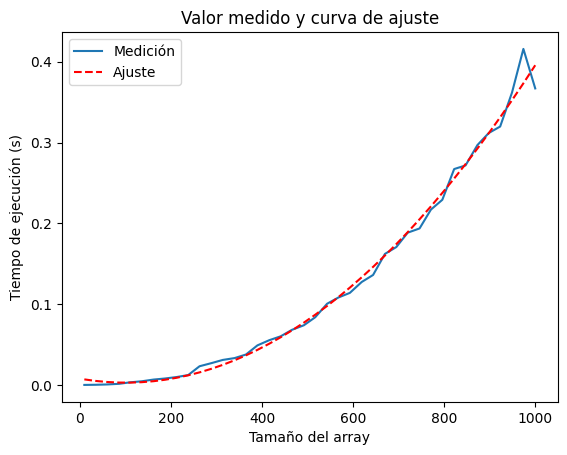
\includegraphics[scale = 0.6]{ {images/cuadradosMinimos.png} }
\end{center}


A simple vista se puede observar un crecimiento $exponencial$. Para confirmar esto, vamos a ajustar los datos a una recta mediante cuadrados mínimos. Esto lo realizamos con \textit{Python} y la función \textit{optimize.curve\_fit} de la biblioteca \textit{scipy}.

Obtenemos que el gráfico se puede ajustar a la curva $y = 1.45e^{-2} \times 2^{x}$, con un error cuadrático medio de $1.485e^{-1}$. Por lo tanto, podemos verificar lo que ya vimos en la sección~\ref{sec:backtracking}, que el orden es exponencial \textbf{O($2^n$)}.

\begin{center}
    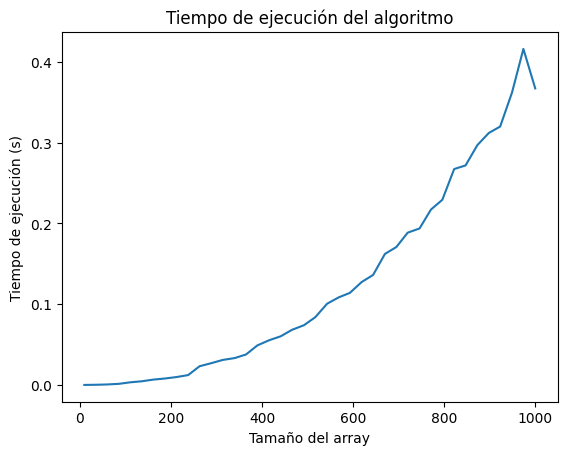
\includegraphics[scale = 0.6]{ {images/image.png} } 
\end{center}